\section{Implementace}
Implementace probíhala v jazyce $C\#$ a vývojovém prostředí Unity3D \cite{Unity}, ve kterém mám dlouholetou zkušenost. 
\subsection{Základní model Boid}
Reynolds ve svém článku neuvádí jakým stylem jednotlivé pravidla řídit ani jaké váhy použít. Byla tedy vytvořena váha pro každé pravidlo, díky kterému můžeme řídit prioritu těchto pravidel. 
\par
Pro lepší vizuální představu jak model Boid funguje byl vytvořen jednoduchý editor, ve kterém je možné v reálném čase nastavit upravit váhy jednotlivým pravidlům a vidět změnu v chování hejna, aniž by bylo potřeba pouštět celou simulaci znovu. To umožnilo rychleji dosáhnout požadovaného chování hejna. Pro správné nastavení vah by teoreticky šel použít i evoluční algoritmus, avšak na tak jednoduchém příkladě není jasné jakým způsobem určovat fitness. 
\par
Podařilo se dosáhnout fungujícího modelu hejna, které však nekontrolovaně cestovalo po světě. 
\subsection{Rozšíření o pravidlo cíle}
Model Boid popisuje pouze chování jednotlivce v hejnu. Pro potřebu kontrolovat pohyb celého hejna, byl agent rozšířen o další pravidlo. Každý agent se snaží dostat do cíle, který je reprezentován pozicí bodu ve světě. 
\par
Od toho pravidla vyžadujeme, ať přitahuje agenta k cíli, ale neznehodnotí zbylé 3 pravidla s narůstající vzdáleností od cíle. Normalizování směrového vektoru k cíli se může zdát jako krok správným směrem. V praxi se však ukázalo, že když je takový agent velmi blízko svého cíle, normalizace vektor naopak zvětší. To má za následek příliš agresivní snahu jedince dostat se do cíle. Proto velikost směrového vektoru od jedince k cíli pouze ořízneme na hodnotu vzdálenosti, od které má být agent méně agresivní. 
\par
Pomocí nového pravidla je možné kontrolovat pozici hejna a pozicovat ho dle svých potřeb. Pro názornou ukázku vznikla scéna s akváriem a rybičkami. V určitém časovém intervalu nastavuji všem agentům (rybám) náhodně vygenerovaný cíl uvnitř akvária.  
\begin{figure}[H]
	\label{fig:ryby_20_50}
	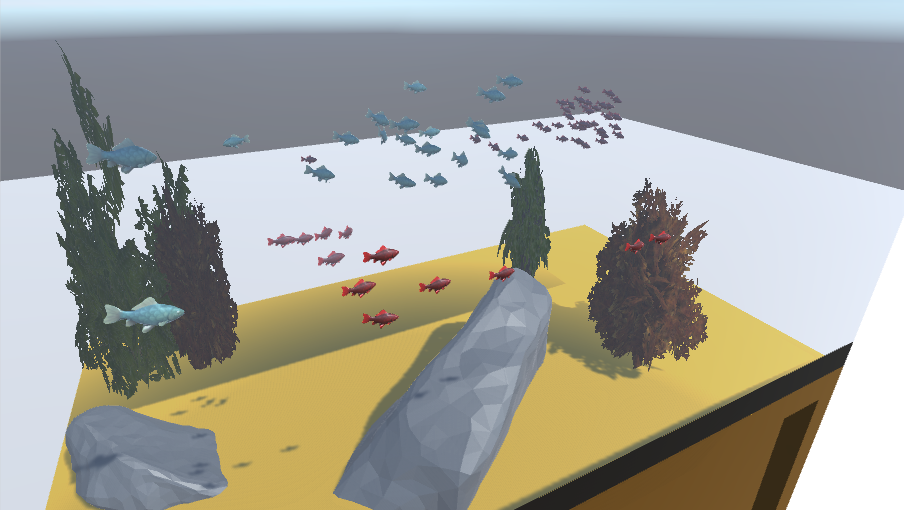
\includegraphics[width=10cm]{fish_20_50.png}
	\centering
	\caption{Hejno 20 modrých a 50 červených ryb}
\end{figure}
Na obrázku \ref{fig:ryby_20_50} můžeme vidět 2 různě početné a nastavené skupiny agentů. První je skupina 20 velkých modrých ryb, které jsou pomalé, drží se dál od sebe (velká váha u separace) a pomalu mění svůj směr. Druhá skupina obsahuje 50 malých červených ryb, které jsou rychlejší, agilnější, ale více se drží pohromadě (velká váha u koheze a vyrovnání). 
\begin{figure}[H]
	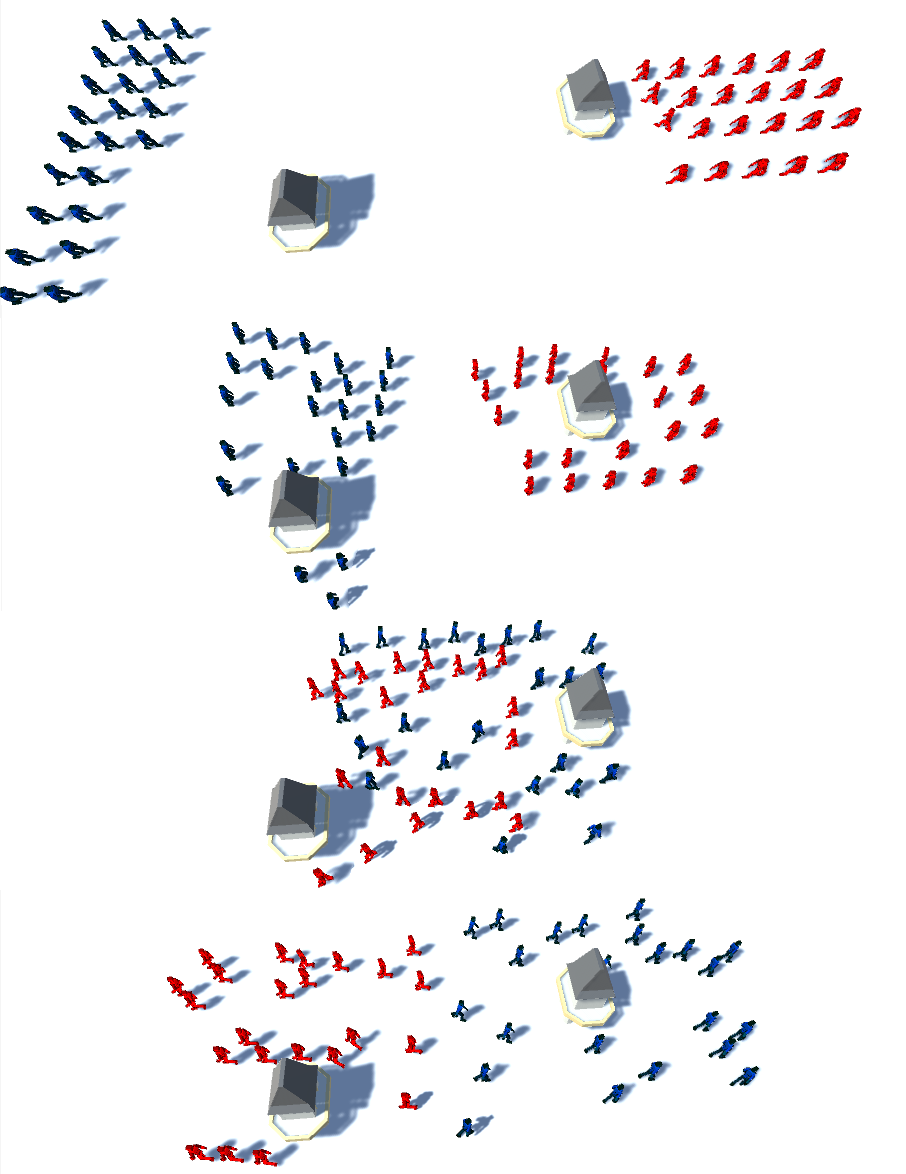
\includegraphics[width=10cm]{peopleAgents_anim.png}
	\centering
	\caption{2 skupiny agentů s detekcí překážek v časech $t=\{ 0,10,20,30\} $}
\end{figure}

Stejnými pravidly se dá simulovat i dav lidí, kteří se potřebují dostat z jednoho místa na druhé. Pro tyto účely byl každému jedinci nastaven odlišný cíl. 


\begin{figure}[H]
	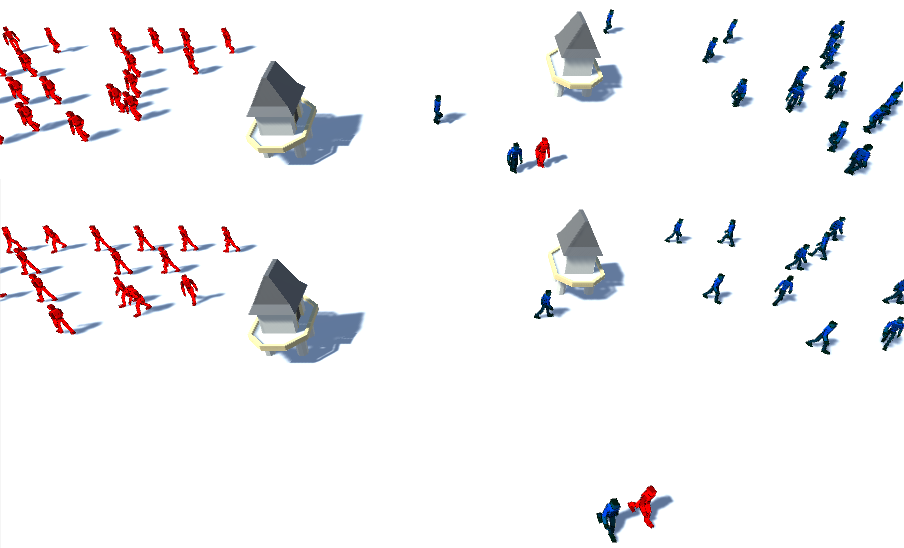
\includegraphics[width=10cm]{people_problem_anim.png}
	\centering
	\caption{Srážka a zamknutí dvou agentů}
\end{figure}

